%
%  Larry Leemis
%
\documentclass[12pt,fullpage]{article}
\usepackage{fullpage}
\usepackage{psfrag}                                          % LaTeX graphics tool
\usepackage{pslatex}                                         % avoids the default cmr font
\usepackage{graphicx}                                        % graphics package 
\usepackage{epsfig} 
\usepackage{hyperref}
\usepackage{color}

\begin{document}

\noindent
{\bf Exponential distribution} (from \color{blue}\url{http://www.math.wm.edu/~leemis/chart/UDR/UDR.html}\color{black})

\noindent
The shorthand $X \sim {\rm exponential}(\alpha)$ is used to indicate
that the random variable $X$ has the exponential distribution with
positive scale parameter $\alpha$.  The exponential distribution can
be parameterized by its {\it mean\/}~{$\alpha$} with the probability density
function
$$
f(x) = \frac{1}{\alpha} e ^ {- x / \alpha} \qquad \qquad x > 0,
$$
for $\alpha > 0$.
An exponential random variable $X$ can also be parameterized by its
{\it rate\/} $\lambda$ via the probability density function 
$$
f(x) = \lambda e ^ {- \lambda x} \qquad \qquad x > 0,
$$
for $\lambda > 0$.
When the second parameterization is used, the meaning of the rate parameter depends
on the application (for example, failure rate for reliability, arrival rate or service rate
for queueing, recidivism rate in criminal justice).
The exponential distribution is used in reliability to model the lifetime of an
object which, in a statistical sense, does not age (for example, a
fuse or light bulb).  This property is known as the memoryless property.
The exponential distribution is the only continuous distribution that
possesses this property.
The only discrete distribution with the memoryless property is the
geometric distribution.
The exponential distribution is used in queueing
theory to model the times between customer arrivals and the service times.
The exponential distribution is used in survival analysis to model
the lifetime of an organism or the survival time after treatment.
The probability density function using the first parametrization with $\alpha = 0.5,\ 1,\ 2$ is illustrated below.

\begin{figure}[h!]
\begin{center}
\psfrag{lab1}{$\alpha = 1$}
\psfrag{lab2}{$\alpha = 2$}
\psfrag{lab3}{$\alpha = 0.5$}
\psfrag{labx}{$x$}
\psfrag{labf}{$f(x)$}
\includegraphics[width=3.2in]{ExponentialPlot.ps}
\end{center}
\end{figure}

\noindent
Using the first parameterization, the cumulative distribution function on
the support of $X$ is
$$
F(x) = P(X \le x) = 1 -  e ^ {- x / \alpha} \qquad \qquad x > 0.
$$
The survivor function on the support of $X$ is
$$
S(x) = P(X \ge x) = e ^ {-x / \alpha} \qquad \qquad x > 0.
$$
The hazard function on the support of $X$ is
$$
h(x) = \frac{f(x)}{S(x)} = \frac{1}{\alpha} \qquad \qquad x > 0.
$$
The cumulative hazard function on the support of $X$ is
$$
H(x) = - \ln S(x) = \frac{x}{\alpha} \qquad \qquad x > 0.
$$
The inverse distribution function of $X$ is
$$
F ^ {-1}(u) = - \alpha \ln (1 - u) \qquad \qquad 0 < u < 1.
$$
The median of $X$ is
$$
\alpha \ln \, 2 .
$$
The moment generating function of $X$ is
$$
M(t) = E\left[ e ^ {tx} \right] = (1 - \alpha\,t)^{-1} \qquad \qquad t < \frac{1}{\alpha}.
$$
The characteristic function of $X$ is
$$
\phi(t) = E\left[ e ^ {itX} \right] =  (1 - \alpha\,it)^{-1} \qquad \qquad t < \frac{1}{\alpha}.
$$
The population mean, variance, skewness, and kurtosis of $X$ are
$$
E[X] = \alpha \qquad \qquad 
V[X] = \alpha^2 \qquad \qquad 
E\left[ \left( \frac{X - \mu}{\sigma} \right) ^ 3 \right] = 2 \qquad \qquad 
E\left[ \left( \frac{X - \mu}{\sigma} \right) ^ 4 \right] = 9.
$$
For $X_1, \, X_2, \, \ldots , \, X_n$ mutually independent exponential($\alpha$) random variables,
the maximum likelihood estimator for $\alpha$ is
$$
\hat \alpha = \frac{\sum_{i\,=\,1}^n X_i}{n},
$$
which is the sample mean.  This is also the method of moments estimator. 
%An exact $(1 - \alpha) \cdot 100$\% confidence interval for $\alpha$ is
%$$
%$$
\vspace{0.1in}

\noindent
{\bf APPL verification:}
The APPL statements
\begin{verbatim}
assume(alpha > 0);
X := [[x -> exp(-x / alpha) / alpha], [0, infinity], ["Continuous", "PDF"]]; 
CDF(X);
SF(X);
HF(X);
CHF(X);
Mean(X);
Variance(X);
Skewness(X);
Kurtosis(X);
MGF(X);
\end{verbatim}
verify the cumulative distribution function, survivor function, hazard function, cumulative hazard function, population mean, variance, skewness, kurtosis, and moment generating function.
\end{document}
